% !TeX spellcheck = en_US
% !TeX encoding = UTF-8 

\documentclass[14pt,a4paper]{extarticle}

\usepackage[english]{babel}
\usepackage[utf8]{inputenc}
\usepackage{setspace} 
\usepackage[a4paper,
	left=30mm,
	right=10mm,
	top=20mm,
	bottom=20mm]{geometry}
\usepackage{amsmath}
\usepackage{amssymb}
\usepackage{amsthm}
\usepackage{graphicx} 
\usepackage{cite}
\usepackage{subfigure}
\usepackage{subcaption}
\usepackage{kprjHSE} 
\usepackage{tikz}
\usetikzlibrary{positioning}
\usepackage{listings}
\usepackage{xcolor,tabularray}
\usepackage{courier}

\lstset{
	frame=single,
	basicstyle=\ttfamily,
	breaklines=true,
	tabsize=4
}

\LabWork
\LabWorkNo{2}

\FirstAuthor{M.D.~Kirdin}
\FirstConsultant{A.~Tomat}
\SecondConsultant{M.~Zueva}
\discipline{Ordered Sets for Data Analysis}
\faculty{Faculty of Computer Science}
\chair{School of Data Analysis and Artificial Intelligence}
\chief{S.O.~Kuznetsov}
\workyear{2024}

\onehalfspacing

\begin{document}
	\maketitle
	
	\subsection*{Question 1}
	\noindent\textbf{Task.} Given the following formal context, find all formal concepts, draw the concept lattice,
	and find all non-trivial implications.
	\begin{center}
	\begin{tblr}{
			width=\linewidth, 
			colspec={|X[c]|X[c]|X[c]|X[c]|X[c]|X[c]|}
			}
		\hline
		 & a & b & c & d & e\\
		\hline
		1 & 1 &  & 1 &  & 1\\
		\hline
		2 & 1 &  & 1 & 1 & \\
		\hline
		3 & 1 &  &  & 1 & 1\\
		\hline
		4 & 1 & 1 &  & 1 & \\
		\hline
		5 & 1 & 1 &  &  & 1\\
		\hline
	\end{tblr}
	\end{center}
	 
	 \noindent\textbf{Solution.} Let the set of all objects be denoted as $G=\{1,\, 2,\, 3,\, 4,\, 5\}$ and the set of all attributes as $M=\{a,\, b,\, c,\, d,\, e\}$. We will condense all the data about formal concepts in this context into a table, where $A \subseteq G$ is set of objects defining a concept.
	 
	 \begin{center}
	 	\begin{tblr}{
	 			width=\linewidth, 
	 			colspec={|X[c]|X[c]|X[c]|X[c]|}
	 		}
	 		\hline
	 		 A & $A^\prime$ & $A^{\prime\prime}$ & Formal concept?\\
	 		\hline
	 		$\{\emptyset_{M}\}$ & $G$ & $\{\emptyset_{M}\}$ & \SetCell{green9} Yes \\
	 		\hline
	 		$M$ & $\{a\}$ & $M$ & \SetCell{green9} Yes \\
	 		\hline
	 		$\{1\}$ & $\{a,\, c,\, e\}$ & $\{1\}$ & \SetCell{green9} Yes \\
	 		\hline
	 		$\{2\}$ & $\{a,\, c,\, d\}$ & $\{2\}$ & \SetCell{green9} Yes \\
	 		\hline
	 		$\{3\}$ & $\{a,\, d,\, e\}$ & $\{3\}$ & \SetCell{green9} Yes \\
	 		\hline
	 		$\{4\}$ & $\{a,\, b,\, d\}$ & $\{4\}$ & \SetCell{green9} Yes \\
	 		\hline
	 		$\{5\}$ & $\{a,\, b,\, e\}$ & $\{5\}$ & \SetCell{green9} Yes \\
	 		\hline
	 		$\{1,\, 2\}$ & $\{a,\, c\}$ & $\{1,\, 2\}$ & \SetCell{green9} Yes \\
	 		\hline
	 		$\{1,\, 3\}$ & $\{a\}$ & $M$ & No \\
	 		\hline
	 		$\{1,\, 4\}$ & $\{a\}$ & $M$ & No \\
	 		\hline
	 		$\{1,\, 5\}$ & $\{a,\, e\}$ & $\{1,\, 3,\, 5\}$ & No \\
	 		\hline
	 		$\{2,\, 3\}$ & $\{a,\, d\}$ & $\{2,\, 3,\, 4\}$ & No \\
	 		\hline
	 		$\{2,\, 4\}$ & $\{a,\, d\}$ & $\{2,\, 3,\, 4\}$ & No \\
	 		\hline

	 	\end{tblr}
	 	\begin{tblr}{
	 			width=\linewidth, 
	 			colspec={|X[c]|X[c]|X[c]|X[c]|}
	 		}
	 		\hline
	 		A & $A^\prime$ & $A^{\prime\prime}$ & Formal concept?\\
	 		\hline
	 		$\{2,\, 5\}$ & $\{a\}$ & $M$ & No \\
	 		\hline
	 		$\{3,\, 4\}$ & $\{a,\, d\}$ & $\{2,\, 3,\, 4\}$ & No \\
	 		\hline
	 		$\{3,\, 5\}$ & $\{a\}$ & $M$ & No \\
	 		\hline
	 		$\{4,\, 5\}$ & $\{a,\, b\}$ & $\{4,\, 5\}$ & \SetCell{green9} Yes \\
	 		\hline
	 		$\{1,\, 2,\, 3\}$ & $\{a\}$ & $M$ & No\\
	 		\hline
	 		$\{1,\, 2,\, 4\}$ & $\{a\}$ & $M$ & No\\
	 		\hline
	 		$\{1,\, 2,\, 5\}$ & $\{a\}$ & $M$ & No\\
	 		\hline
	 		$\{2,\, 3,\, 4\}$ & $\{a,\, d\}$ & $\{2,\, 3,\, 4\}$ & \SetCell{green9} Yes\\
	 		\hline
	 		$\{2,\, 3,\, 5\}$ & $\{a\}$ & $M$ & No\\
	 		\hline
	 		$\{3,\, 4,\, 5\}$ & $\{a\}$ & $M$ & No\\
	 		\hline
	 		$\{1,\, 2,\, 3,\, 4\}$ & $\{a\}$ & $M$ & No\\
	 		\hline
	 		$\{1,\, 2,\, 3,\, 5\}$ & $\{a\}$ & $M$ & No\\
	 		\hline
	 		$\{1,\, 2,\, 4,\, 5\}$ & $\{a\}$ & $M$ & No\\
	 		\hline
	 		$\{1,\, 3,\, 4,\, 5\}$ & $\{a\}$ & $M$ & No\\
	 		\hline
	 		$\{2,\, 3,\, 4,\, 5\}$ & $\{a\}$ & $M$ & No\\
	 		\hline
	 	\end{tblr}
	 \end{center}
	 Having found all the formal concepts, we are able to construct the concept lattice.
	 
	 \begin{center}
	 \resizebox{\linewidth}{10em}{%
	 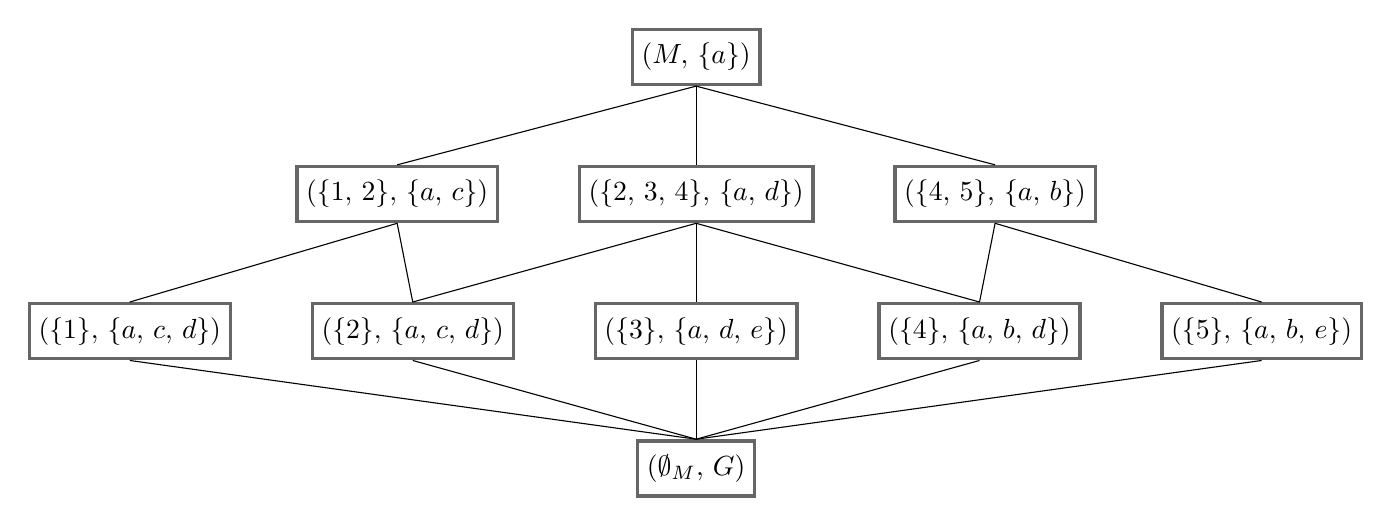
\begin{tikzpicture}[
	 	squarednode/.style={rectangle, draw=black!60, very thick, minimum size=7mm},
	 	]
	 	%Nodes
	 	\node[squarednode]      (toplayer)   {$(M,\, \{a\})$};
	 	\node[squarednode]      (3layer2)    [below=of toplayer] {$(\{2,\, 3,\, 4\},\, \{a,\, d\})$};
	 	\node[squarednode]      (3layer3)    [right=of 3layer2] {$(\{4,\, 5\},\, \{a,\, b\})$};
	 	\node[squarednode]      (3layer1)    [left=of 3layer2] {$(\{1,\, 2\},\, \{a,\, c\})$};
	 	\node[squarednode]      (2layer3)    [below=of 3layer2] {$(\{3\},\, \{a,\, d,\, e\})$};
	 	\node[squarednode]      (2layer2)    [left=of 2layer3] {$(\{2\},\, \{a,\, c,\, d\})$};
	 	\node[squarednode]      (2layer4)    [right=of 2layer3] {$(\{4\},\, \{a,\, b,\, d\})$};
	 	\node[squarednode]      (2layer1)    [left=of 2layer2] {$(\{1\},\, \{a,\, c,\, d\})$};
	 	\node[squarednode]      (2layer5)    [right=of 2layer4] {$(\{5\},\, \{a,\, b,\, e\})$};
	 	\node[squarednode]      (bottomlayer)    [below=of 2layer3] {$(\emptyset_{M},\, G)$};
	 	
	 	%Lines
	 	\draw[-] (toplayer.south) -- (3layer3.north);
	 	\draw[-] (toplayer.south) -- (3layer2.north);
	 	\draw[-] (toplayer.south) -- (3layer1.north);
	 	\draw[-] (3layer1.south) -- (2layer1.north);
	 	\draw[-] (3layer1.south) -- (2layer2.north);
	 	\draw[-] (3layer2.south) -- (2layer2.north);
	 	\draw[-] (3layer2.south) -- (2layer3.north);
	 	\draw[-] (3layer2.south) -- (2layer4.north);
	 	\draw[-] (3layer3.south) -- (2layer4.north);
	 	\draw[-] (3layer3.south) -- (2layer5.north);
	 	\draw[-] (2layer1.south) -- (bottomlayer.north);
	 	\draw[-] (2layer2.south) -- (bottomlayer.north);
	 	\draw[-] (2layer3.south) -- (bottomlayer.north);
	 	\draw[-] (2layer4.south) -- (bottomlayer.north);
	 	\draw[-] (2layer5.south) -- (bottomlayer.north);
	 \end{tikzpicture}
	}
	 \end{center}
	 \newpage
	 
	 \subsection*{Question 2}
	 
	 \noindent\textbf{Task.} Using the diagram find:
	 \begin{enumerate}
	 	\item $f\land m,\, a\lor l,\, i \land k$;
	 	\item $a\land(c\lor d),\, (i\land g)\lor(c\land d),\, \lor(b,\, c,\, d)$;
	 	\item $\land \varphi,\, \lor \varphi$;
	 \end{enumerate}
	 and determine whether the diagram represents an upper semi-lattice, a lower semi-lattice or a lattice.
	 
	 \begin{figure}[h]
	 	\includegraphics[scale=1.0]{media/task2.png}
	 	\centering
	 \end{figure}
	 
\end{document}